\documentclass{article}
\usepackage[utf8]{inputenc}
\usepackage{float}
\usepackage{graphicx}

\title{DB}
\author{Ahmad Agung Tawakkal\\1184015\\D4 TI 1B}
\date{October 2019}

\graphicspath{{images/}}

\begin{document}

\maketitle

\newpage

\paragraph{}Apex (App Express) merupakan aplikasi WEB BASED, WEB BASED adalah aplikasi yang dibuat berbasis web yang membutuhkan web server dan browser untuk menjalankan. Apex Sendiri tidak membutuhkan perangkat lain untuk pengembangan kerna app apex telah memiliki fitur sebagai berikut;
    \begin{itemize}
        \item App Builder 
            \paragraph{}App builder dapat membuat, melihat, mengimport, mengatur service, mengatur user aplikasi dan memantau aktifitas dari penggunanya sendiri.
        \item SQL Workshop
            \paragraph{}SQL workshop dapat membuat table menggunakan perintah SQL, SQL (STRUKTUR QUERRY LENGUAGE) adalah bahasa pemrograman untuk mengelolah data maupun membuat data. SQL juga dapat melihat sruktur dari data tabel yang telah ada dan lain-lain.
        \item Utilitas 
            \paragraph{}Dapat meilihat report tabel dan komponennya serta history aplikasi.
    \end{itemize}
    
\begin{enumerate}
    \item Membuat Aplikasi
        \begin{itemize}
            \item Buka link https://apex.oracle.com/pls/apex/f?p=4700:2:113057905128983::NO:RP::
            \item Mengisi data yang yang dibutuhkan untuk request pembuatan workspace,
            \item Jika telah selesai memasukkan data yang diminta selanjuntya tekan submit request.
            \item Kemudian akan ada pemeberitahuan dari oracle ke email anda untuk mengkonfirmasi
            \item Jika anda ingin menkonfirmasi anda harus memasukkan password untuk konfigurasi.
            \item Jika telah selesai anda login ke apex.
            \item Pada menu utama anda tekan app bilder.
            \item Kemudian pilih Creat a new application.
            \item New application
            \item Masukkan nama App.
            \item Centang semua pada fiturnya.
            \item Kemduian pilih create app.
            \item Tunggu prosesnya sampai selesai.
            \item Jika telah selesai anda tinggal klik Run untuk menjalangkan App yang telah dibuat.
            \item Maka akan muncul tampilan sebagi berikut.
                \begin{figure}
                    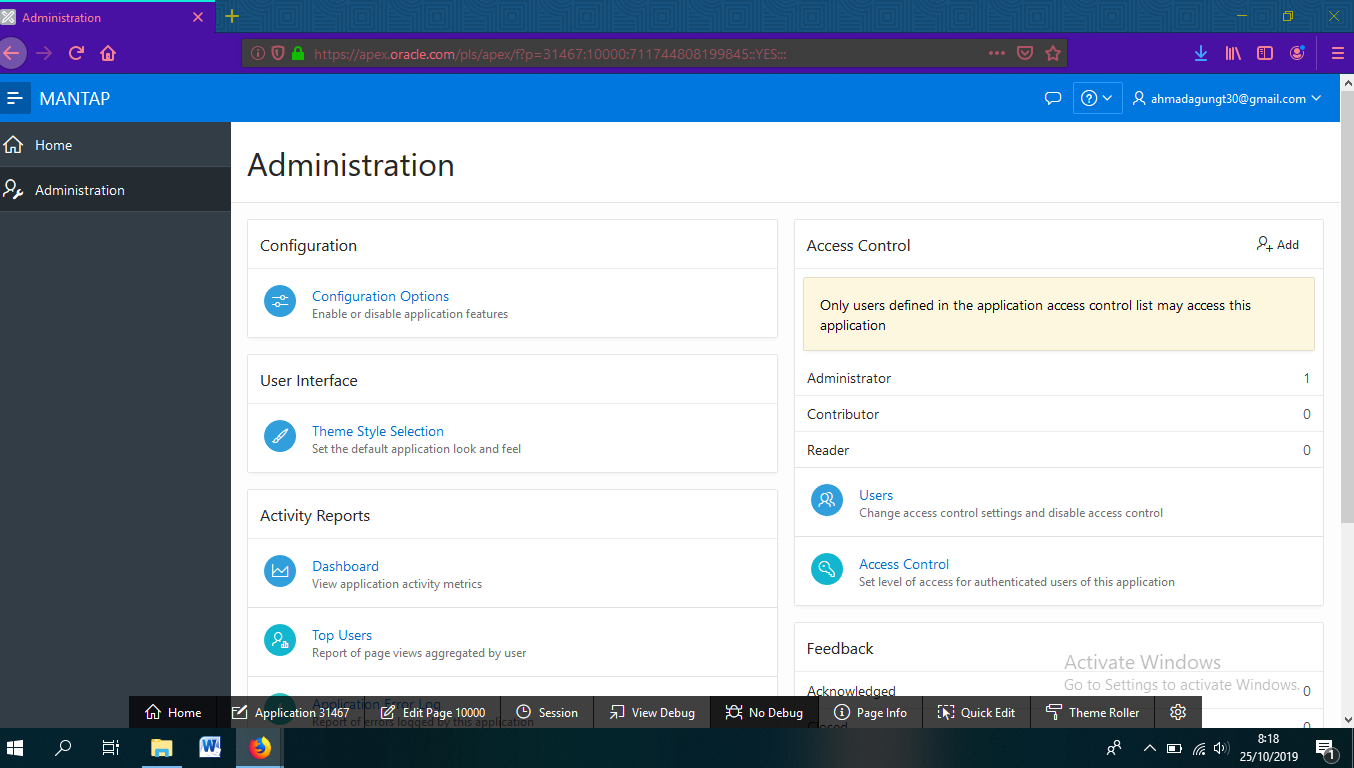
\includegraphics[width=15cm]{1.PNG}
                \end{figure}
        \end{itemize}
    \paragraph{} Jadi App Builder berguna untuk membuat aplikasi yang berhubungan dengan database dan tersimpan sebagai skema didalam aplikasi oracle express.
\end{enumerate}

\end{document}
